\section{Data Analyses} \label{sec:Data Analyses}
    \subsection{Computational Analysis}
        We then choose a damping coefficient ($b=0.4$) and a torsion coefficient ($\kappa = .1$) and then run the RK4 simulator for the experimentally measured angles ($125, 90, 60, 45, 30, 15, 0$). Using the numpy's real Fast Fourier Transform (numpy.fft.rfft()). We find that the $c_0$ for each initial angle: 
        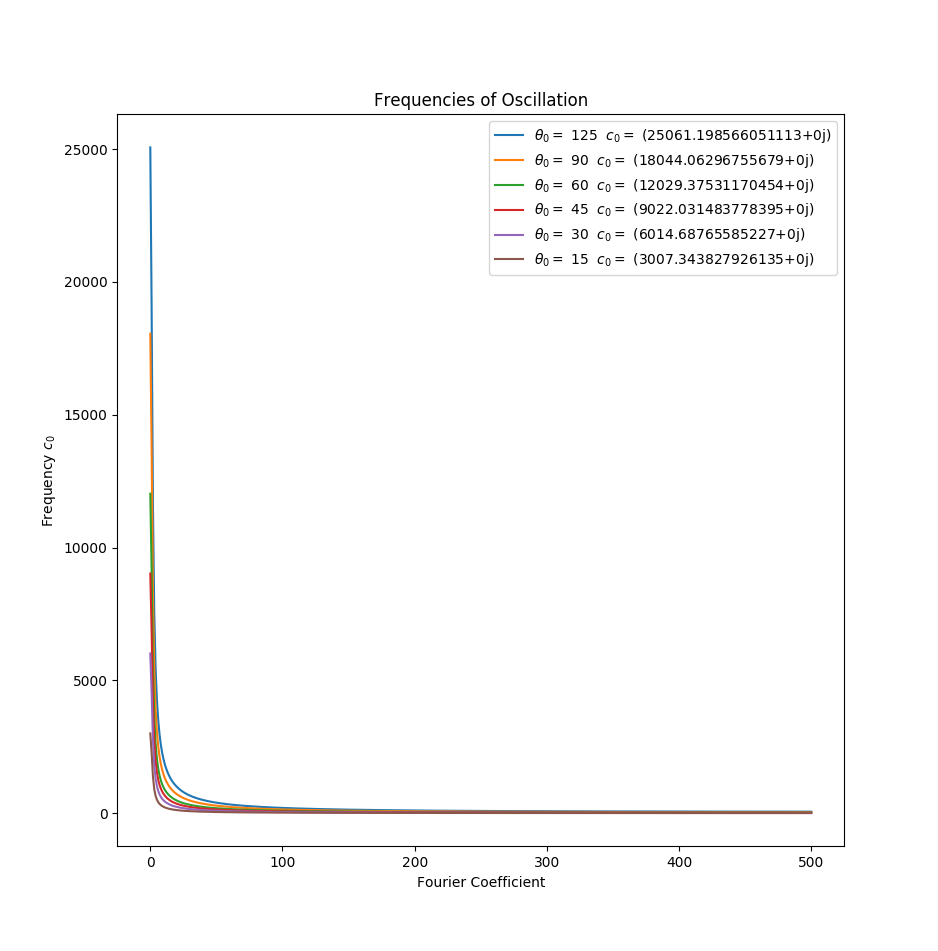
\includegraphics[width=\linewidth]{figures/Figure 3 - Angular Frequancies .png}
        Then we can find that the angular phase portrait for each initial angle is given as: 
        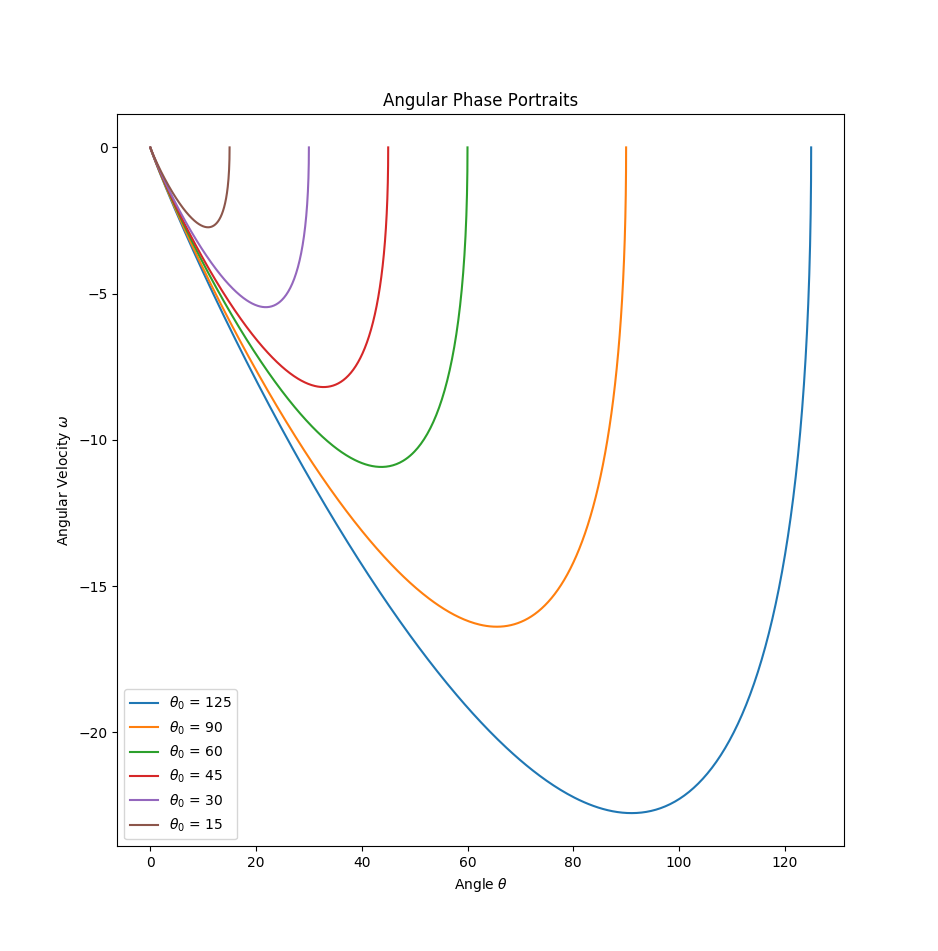
\includegraphics[width=\linewidth]{figures/Figure 4 - Angular Phase Portrait.png}
    \subsection{Experimental Analysis}
        For the measurement of the force, we (unfortunately) were only able to measure in pounds, so later we convert to Newtons. The tick marks were at each whole pound, so any decimal is an estimation. The door showed having a consistent 2.0lb of force (pounds are force in imperial units, luckily, and fun fact, the "slug" is the imperial unit of mass) when opened as described in the procedure above. When receding back to zero, however, we note that in-between the 60° and 45°markings, the force dropped from 2.0lb to roughly 1.2lb. We continued to read this measurement until the door hit something like a "release" in between 15° and 7° (in fact, it was after noticing this that we chose to include the angle measurement at 7°), where the reading evidently jumped back up to 1.6lb.\par
        For the angle versus time measurements, we have included all our recorded data as seen in Table I. Further we have used MATLAB to plot the angle versus time scatter plot in Figures 3 (a), and the angular velocity and angular acceleration plots Figure 3 (b)-(c).
        \begin{center}
            \begin{table}
            \begin{tabular}{||c || c c c c c||} 
            \hline
            Angle range & Trial 1 & Trial 2 & Trial 3 & Trial 4 & Trial 5\\ [0.5ex] 
            \hline\hline
             125°-90° & 1.48s &  1.42s & 1.48s & 1.39s & 1.5s \\ 
            \hline
            90°-60° & 1.93s & 1.95s & 2.09s & 1.90s & 1.89s \\
            \hline
            60°-45° & 5.58s & 5.32s & 5.92s & 5.30s & 5.41s \\
            \hline
             45°-37° & 8.15s & 6.90s & 7.60s & 6.73s & 6.83s \\
            \hline
            37°-30° & 12.75s & 12.41s & 11.76s & 11.14s & 11.49s \\ 
            \hline
            30°-15° & 21.68s & 19.61 & 19.03s & 19.50s & 20.12s\\
            \hline
            15°-7° & 26.37s & 25.42 & 24.56s & 24.09s & 25.05s\\ [1ex] 
            \hline
            \end{tabular}
            \caption{Data collected from a screen door with manual closer}
            \label{table:1}
            \end{table}
        \end{center}
        \begin{figure}[htbp]
        \centering
        \subfloat[Angle vs. Time plot]{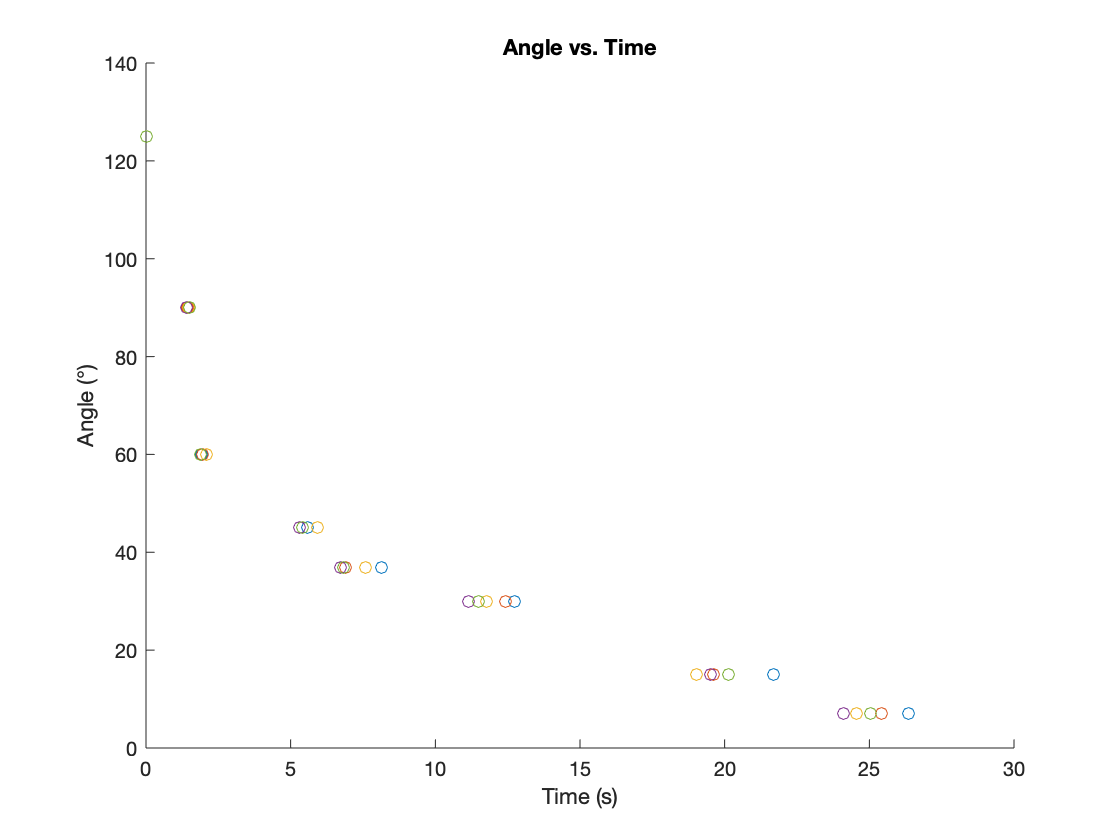
\includegraphics[width=\linewidth]{figures/Figure 3a - Angle vs Time.png}}\\
        \subfloat[Angular Velocity vs. Time plot]{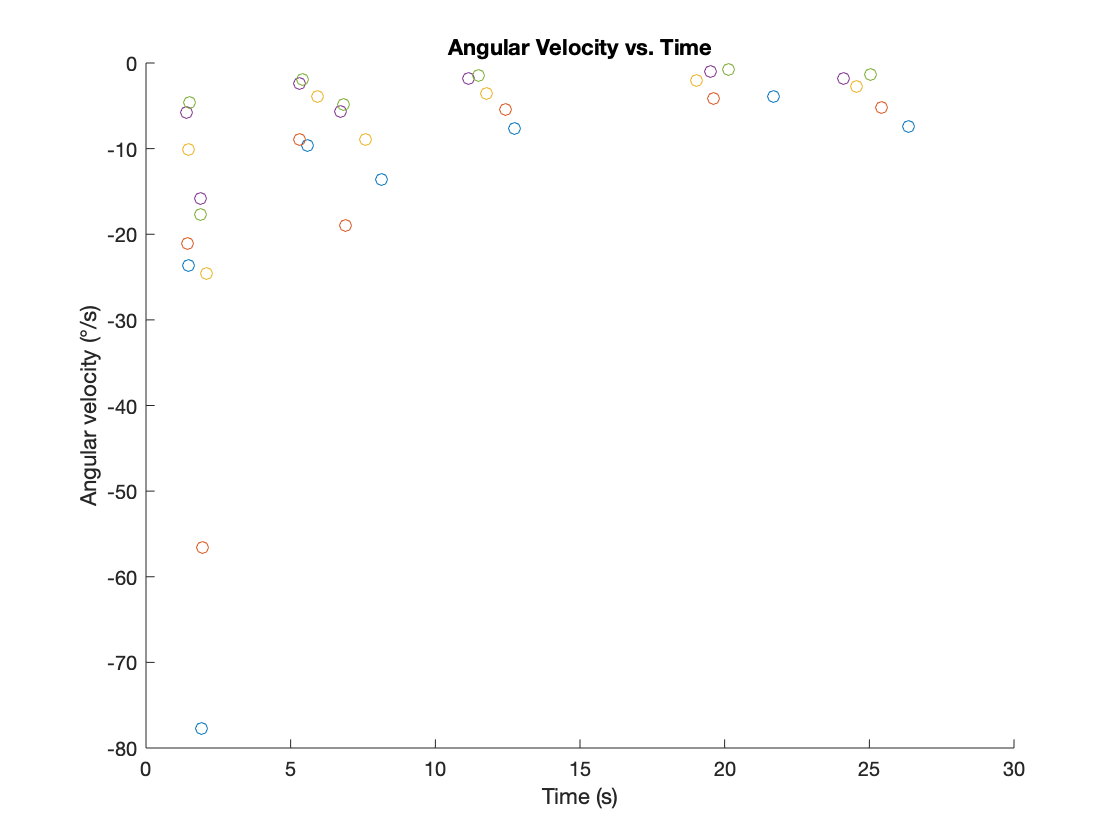
\includegraphics[width=\linewidth]{figures/Figure 3b - Angular Velocity vs Time.png}}\\
        \subfloat[Angular Acceleration vs. Time plot]{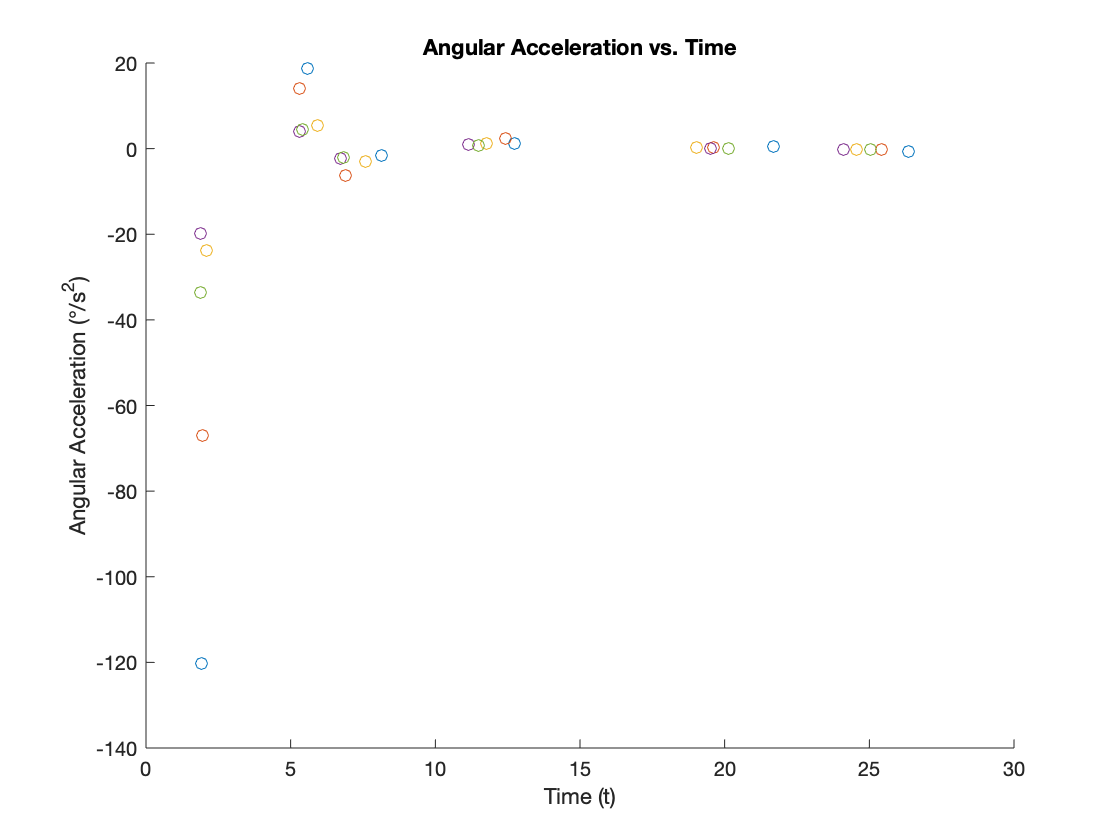
\includegraphics[width=\linewidth]{figures/Figure 3c - Angular Acceleration vs Time.png}}
        \caption{MATLAB plots for experimental results}
        \end{figure}\par
        Notice that in the Figure 3a , the first three points resemble that of a negative quadratic function of time ($-t^{2}$), but then the rest of the points appear to correlate more with an negative exponential function of time ($e^-{t}$) as in our overdamped and critically damped cases. We note that from our formalism, an undamped case for the function of the angle with time would resemble a cosine funtion, and when approximated to the second degree Taylor polynomial, this cosine function is in fact a dominated by a negative quadratic. Thus we would expect that for those first three points (roughly), our manual closer provided no damping, and after the third point the closer began to apply some retarding force. Both of these are fully consistent with the force measurements which we have taken. \par
        Further, note that towards the final points on Figure 3 (b) and (c) that the angular velocity and angular accelerations decrease (with respect to an opening frame of reference). As we have previously mentioned, the door seemed to have some release mechanism towards the smallest angles where, the force seemed to spike back up. These changes in the angular velocities and angular accelerations (though minuscule) show this phenomenon quite nicely.
        